%%%%%%%%%%%%%%%%%%%%%%%%%%%%%%%%%%%%%%%%%%%%%%%%%%%%%%%%%%%%%%%%%%%%%%%%%%%%
% AGUJournalTemplate.tex: this template file is for articles formatted with LaTeX
%
% This file includes commands and instructions
% given in the order necessary to produce a final output that will
% satisfy AGU requirements, including customized APA reference formatting.
%
% You may copy this file and give it your
% article name, and enter your text.
%
% guidelines and troubleshooting are here: 

%% To submit your paper:
\documentclass[draft]{agujournal2019}
\usepackage{url} %this package should fix any errors with URLs in refs.
\usepackage{lineno}
\usepackage[inline]{trackchanges} %for better track changes. finalnew option will compile document with changes incorporated.
\usepackage{soul}
\usepackage{amsmath}
\usepackage{amssymb}
\usepackage{amsthm}
\usepackage{booktabs}
\usepackage{subcaption}
\usepackage{mathtools}
\linenumbers

\draftfalse

\journalname{Earth and Space Science}


\begin{document}

\title{Calibration and Downscaling of MERRA-2 Reanalysis Data for Improved Air Quality Assessments}

\section{Calibration Written}

\subsection{Data}

As stated in the paper by Sayeed et al. (2022), the MERRA-2 aerosol variables are shown to be biased from the true measurements. Hence, in order to ensure the downscaling variables are accurate, we proposed to include a calibration phase where we used ground-level measurements of PM2.5 as a golden standard to calibrate the MERRA-2 variables for better downscaling quality.

Overall, the calibration phase of this project consists of mainly two datasets, as described below.

\subsubsection{OpenAQ}

OpenAQ is a non-profit organization providing universal access to air quality data, particularly PM2.5 data that we were interested in. In our study region, there are 11 measurement sites in total, all of which are U.S. embassies scattered in Southwest Asia. A list of the locations is included in the appendix. Overall, we gathered over 300,000 PM2.5 hourly measurements in the region from 2016 to 2024.

\subsubsection{MERRA-2}

The Modern-Era Retrospective Analysis for Research and Applications, Version 2, or MERRA-2 for short, is a worldwide reanalysis dataset provided by NASA for environmental studies. The MERRA-2 is a large, comprehensive dataset, and we only used a small subset of all the MERRA-2 variables. The full list of MERRA-2 variables used in this project along with their descriptions is included in the appendix. For this project, the data we selected comes in hourly format to match the OpenAQ PM2.5 measurements.

According to NASA, the mathematical relation between PM2.5 and the MERRA-2 aerosol variables can be summarized by the following equation:
\[\text{PM}_{2.5} = \text{DUST}_{2.5} + \text{SS}_{2.5} + \text{BC} + \text{OC} + 1.375 \times \text{SO}_4\]
As mentioned previously, this equation is empirically shown to be biased. Therefore, we aimed to find a better mathematical relation between PM2.5 and the MERRA-2 variables by fitting some machine learning models.

\subsection{Methodology}

Upon extracting the OpenAQ and MERRA-2 data, some preprocessing was completed. Specifically, since both the PM2.5 measurements and MERRA-2 come in hourly format, we joined the two datasets by matching the date and time at which the measurements were taken so that our models could use the MERRA-2 data to predict the PM2.5 value at the corresponding time step. Additionally, to exploit the temporal nature of environmental data, further data preprocessing included adding temporal lags of MERRA-2 variables in the previous 24 hours for the sake of building models that take advantages of this time series, such as LSTMs and transformers.

In the model fitting stage, we first referenced the methodology conducted by Sayeed et al. (2022) and attempted to replicate the results. We randomly selected 10\% of all the PM2.5 measurements and fit various machine learning models to predict PM2.5 values based on the MERRA-2 data. The full list of machine learning models trained in this part is included in the appendix as well as in the next section. The XGBoost model was trained using the \texttt{XGBoost} library, the neural network using \texttt{PyTorch}, and other models using \texttt{scikit-learn} all with the default hyperparameters. Root mean squared error, or RMSE, was used for evaluation. This step aimed to ascertain the model that has the most potential in the calibration task, while keeping the validation process at a manageable level. The results will be discussed in the subsequent section.

After determining the best model, the entire dataset of all the PM2.5 measurements were split into a training set and a validation set with a 90:10 ratio. The best model type was then fit using the training set along with hyperparameter tuning based on the validation set. Root mean square error was again used as the evaluation metric. Feature engineering was applied, aiming to improve model performance.

In addition to hyperparameter tuning, different neural network architectures were considered during the model training process. Since the MERRA-2 data is essentially an hourly time series, LSTMs and transformers that are designed to handle sequential data were included as building blocks in the final neural network architecture. Furthermore, variational autoencoders or VAEs that aim to model the underlying distribution of the PM2.5 measurements were also part of the experiment during the calibration phase along with transfer learning, a powerful technique for training neural networks. Lastly, multiple loss functions such as mean squared error (MSE), mean absolute error (MAE), huber loss, and quantile loss for quantile regression were compared.

Upon finishing the training phase, the final model was validated on a dataset of PM2.5 measured daily in Kuwait in the 2004-2005 period. This validation step serves to evaluate the generalizability of the model outside of the available time range of the training data and is crucial since the overall objective of the project is to downscale the MERRA-2 components in the 2002-2016 period.

\subsection{Results \& Discussion}

\subsubsection{Subset Validation}

As mentioned in the previous section, various machine learning models have been fit and validated on a 10\% subset of all the available PM2.5 measurements. RMSE was used as the evaluation metric for this part. The results of the subset validation are shown in \textit{Table \ref{tab:subset_eval}} below.

\begin{table}[htbp]
    \centering
    \begin{minipage}{0.48\linewidth}
        \centering
        \begin{tabular}{l c}
            \toprule
            \textbf{Model} & \textbf{Validation RMSE} \\
            \midrule
            Baseline & 51.166 \\
            OLS & 47.841 \\
            Ridge & 49.483 \\
            Lasso & 50.444 \\
            SGD & \(1.680\times 10^{18}\) \\
            KNN & 53.526 \\
            SVM & 52.697 \\
            \bottomrule
        \end{tabular}
    \end{minipage}
    \quad
    \begin{minipage}{0.48\linewidth}
        \centering
        \begin{tabular}{l c}
            \toprule
            \textbf{Model} & \textbf{Validation RMSE} \\
            \midrule
            AdaBoost & 128.360 \\
            GB & 45.063 \\
            HistGB & 43.048 \\
            DT & 62.082 \\
            \textbf{RF} & \textbf{42.246} \\
            \textbf{XGB} & \textbf{43.971} \\
            \textbf{NN} & \textbf{44.113} \\
            \bottomrule
        \end{tabular}
    \end{minipage}
    \caption{Subset Evaluation}
    \label{tab:subset_eval}
\end{table}

From \textit{Table \ref{tab:subset_eval}} above, we see that the models having the lowest validation RMSE on the 10\% subset are random forest, XGBoost, and neural network. These results mostly agreed with the results obtained by Sayeed et al. (2022). Note that HistGB has an even lower validation RMSE than XGBoost and neural network. However, considering that XGBoost is a more powerful model and a superset of HistGB, we decided to move forward with XGBoost instead of HistGB.

\subsubsection{One-Step Prediction}

As stated in the methodology section, two types of data preprocessing were done. One of them was matching the date and time of the PM2.5 measurements and MERRA-2 and using MERRA-2 to predict the PM2.5 value at the corresponding time step. For this part, we trained various fully-connected neural networks by experimenting different sets of hyperparameters. We also applied feature engineering by adding cyclical encodings for date and time, incorporating embedding layers for sites and seasons. Since our study region contains some countries in the Middle East which belong to a region that is more arid than other countries, embeddings for aridity were as well considered. As we added more features, the validation RMSE of the neural networks gradually decreased and is shown in \textit{Table \ref{tab:rmse}} below.

Additionally, as mentioned, random forest and XGBoost were the other two types of models that have shown potentials in this calibration task. Therefore, we made some efforts in fitting these models and tuning the hyperparameters for them. The results with comparison to the final neural network are shown in \textit{Table \ref{tab:model_type}} below.

\begin{table}[htbp]
    \centering
    \begin{minipage}{0.48\linewidth}
        \begin{tabular}{l c}
            \toprule
            \textbf{Data} & \textbf{Validation RMSE} \\
            \midrule
            Only MERRA-2 & 38.184 \\
            Cyclical Encoding & 35.665 \\
            Time \& Site & 36.810 \\
            Site Embeddings & 29.343 \\
            All Embeddings & 26.210 \\
            Aridity & 25.652 \\
            \textbf{Fine-tuned} & \textbf{24.393} \\
            \bottomrule
        \end{tabular}
        \caption{RMSE at Different Stages}
        \label{tab:rmse}
    \end{minipage}
    \quad
    \begin{minipage}{0.48\linewidth}
        \begin{tabular}{l c}
            \toprule
            \textbf{Model} & \textbf{Validation RMSE} \\
            \midrule
            \textbf{Neural Network} & \textbf{24.393} \\
            XGBoost & 25.907 \\
            Random Forest & 40.674 \\
            \bottomrule
        \end{tabular}
        \caption{Model Type Comparison}
        \label{tab:model_type}
    \end{minipage}
\end{table}

From the tables above, we observed that the fine-tuned neural network obtained the lowest validation RMSE of 24.393, outperforming the XGBoost model and the random forest. This is expected as neural networks are a comprehensive set of models that can learn arbitrary non-linear functions well and thus have great potentials. As shown in \textit{Table \ref{tab:rmse}}, we also see that more added features also led to lower validation RMSE. The final model thus had embeddings for sites, seasons, and aridity.

It is worth to note that in the paper by Sayeed et al. (2022), the former researchers successfully achieved a validation RMSE of 7.15 on their random forest. This shows that there is still a large gap in the performance between our random forest and the previous successful model. An observation, though, on our current study is that the region of interest is Southwest Asia instead of the U.S. in the literature. This factor poses a significant challenge because Southwest Asia, especially the Middle East region, is an area that is much more arid than the U.S, and thus originally has PM2.5 measurements that are highly variable. It is obvious that the prediction task should be more difficult in the current study.

\subsubsection{Evaluation \& Limitations}

To better understand the unsatisfactory performance of the models, we made some efforts to evaluate and diagnose our fine-tuned neural network above. Since we had 11 sites in total, we first tried leave-one-out cross validation -- by fitting the model on 10 of the 11 sites and validating it on the last one. We iteratively applied this technique on all 11 sites and obtained the following results as shown in \textit{Table \ref{tab:loo-cv}}.

\begin{table}[htbp]
    \centering
    \begin{tabular}{l c c}
        \toprule
        \textbf{Site} & \textbf{Training RMSE} & \textbf{Validation RMSE} \\
        \midrule
        Baghdad Airnow & 8.8 & 45.0 \\
        \textbf{Baghdad Embassy} & \textbf{8.7} & \textbf{55.4} \\
        Bahrain & 8.2 & 44.2 \\
        Doha & 8.5 & 33.0 \\
        Dubai & 8.1 & 36.5 \\
        \textbf{Kuwait} & \textbf{7.5} & \textbf{51.3} \\
        Kyrgyzstan & 8.1 & 33.7 \\
        Tajikistan Dushanbe & 8.4 & 32.9 \\
        Tajikistan Embassy & 7.9 & 43.8 \\
        Turkmenistan & 8.5 & 44.2 \\
        Uzbekistan & 8.5 & 39.2 \\
        \bottomrule
    \end{tabular}
    \caption{Leave-One-Out Cross Validation}
    \label{tab:loo-cv}
\end{table}

From \textit{Table \ref{tab:loo-cv}}, notice that the neural network is capable of fitting the PM2.5 values well, as shown by the low training RMSE. However, the model failed to generalize to unseen data, and is particularly seen when Baghdad Embassy or Kuwait was left out. This supported our earlier claim that arid areas pose are more problematic when it comes to predicting PM2.5 -- these two sites are located in the Middle East, an area much more arid than others.

Besides leave-one-out cross validation, we also tried plotting the expected PM2.5 measurements vs. the predicted PM2.5 values and the plots are shown in \textit{Figure \ref{fig:eval}} below.

\begin{figure}[htbp]
    \begin{subfigure}[b]{0.48\textwidth}
        \centering
        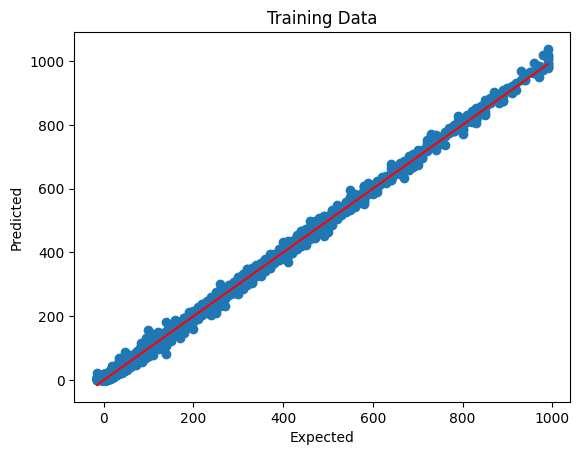
\includegraphics[width=\textwidth]{calibration/training_eval.png}
        \caption{Training, \(R^2 = 0.997\)}
    \end{subfigure}
    \hfill
    \begin{subfigure}[b]{0.48\textwidth}
        \centering
        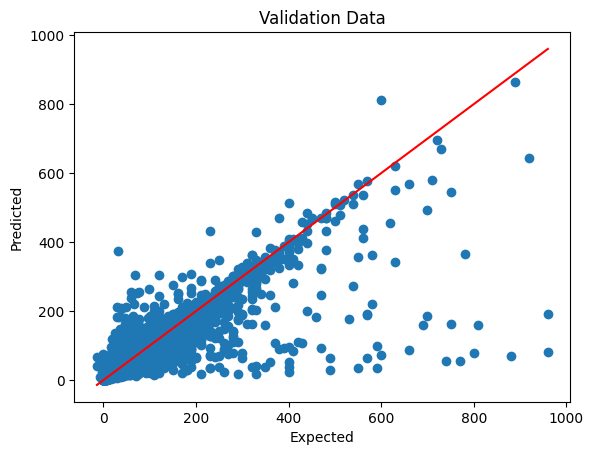
\includegraphics[width=\textwidth]{calibration/validation_eval.png}
        \caption{Validation, \(R^2 = 0.769\)}
    \end{subfigure}
    \caption{Expected vs. Predicted PM2.5 Values}
    \label{fig:eval}
\end{figure}

From the figure, we see that the neural network was fitting the training data very well, proven by the training \(R^2\) value and the straight line in the plot. However, the validation plot looks much more scattered. Particularly, the model seemed to constantly underestimate PM2.5 values that were expected to be greater than 500 \( \mu g/m^3 \), leading to the high validation RMSE. The following section thus describes how we attempted to alleviate this bottleneck by introducing more neural network architectures.

Since the model was constantly underestimating high PM2.5 values, we were curious of whether high PM2.5 values were common in the dataset and so we conducted a diagnostic for summary statistics. \textit{Figure \ref{fig:summary_stats}} below shows the boxplots of the PM2.5 ground measurements classified by measurement sites.

\begin{figure}[htbp]
    \centering
    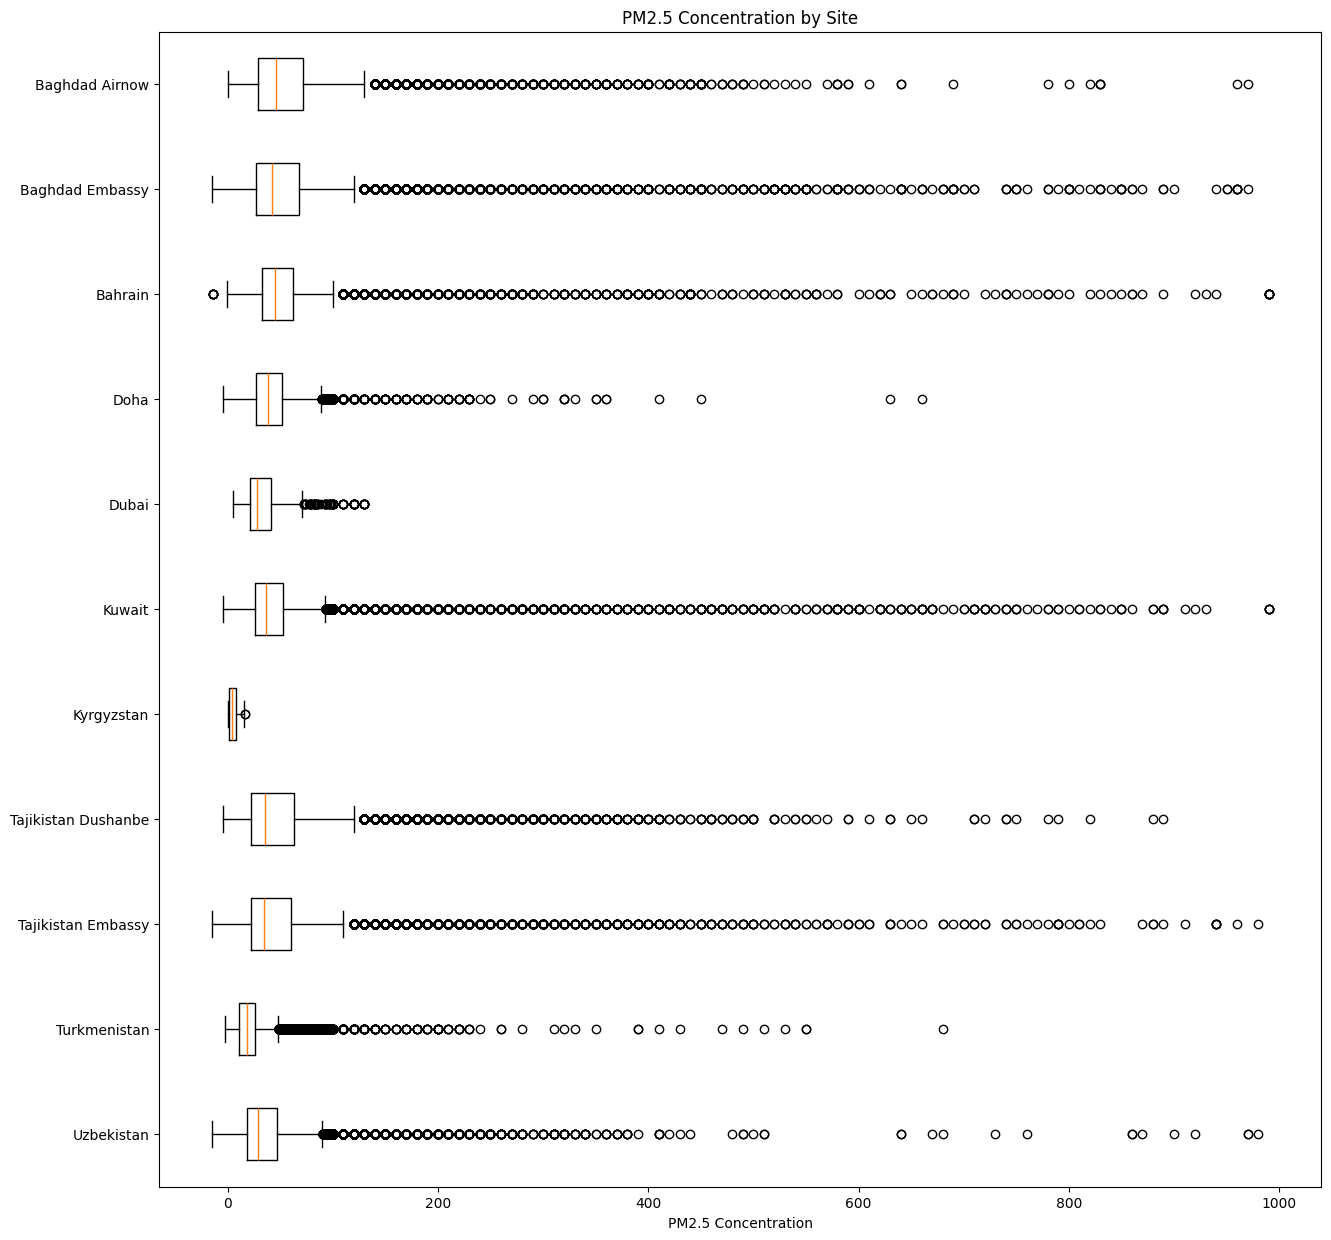
\includegraphics[width=\textwidth]{calibration/summary_stats_boxplots.png}
    \caption{PM2.5 Concentration by Sites}
    \label{fig:summary_stats}
\end{figure}

Note that other than Kyrgyzstan, all other measurement sites have a large number of outliers that have PM2.5 values greater than 100 \( \mu g/m^3 \), while the majority of values fall below the 100 \( \mu g/m^3 \) mark. This supports that the model had difficulties making high PM2.5 predictions since there was not much data to train on. On the other hand, it was not surprising that Kyrgyzstan had the lowest validation RMSE in the leave-one-out practice because there weren't too many outliers associated with this measurement site, thus easier to generalize.

Besides the above observations, we also conducted some additional data diagnostics for the MERRA-2 data. Looking at the full list of the chosen MERRA-2 variables, note that there are some pairs of variables that look similar, such as \texttt{SSSMASS} and \texttt{SSSMASS25}. Therefore, we plotted the correlation plot of the MERRA-2 variables in \textit{Figure \ref{fig:correlations}} below.

\begin{figure}[htbp]
    \centering
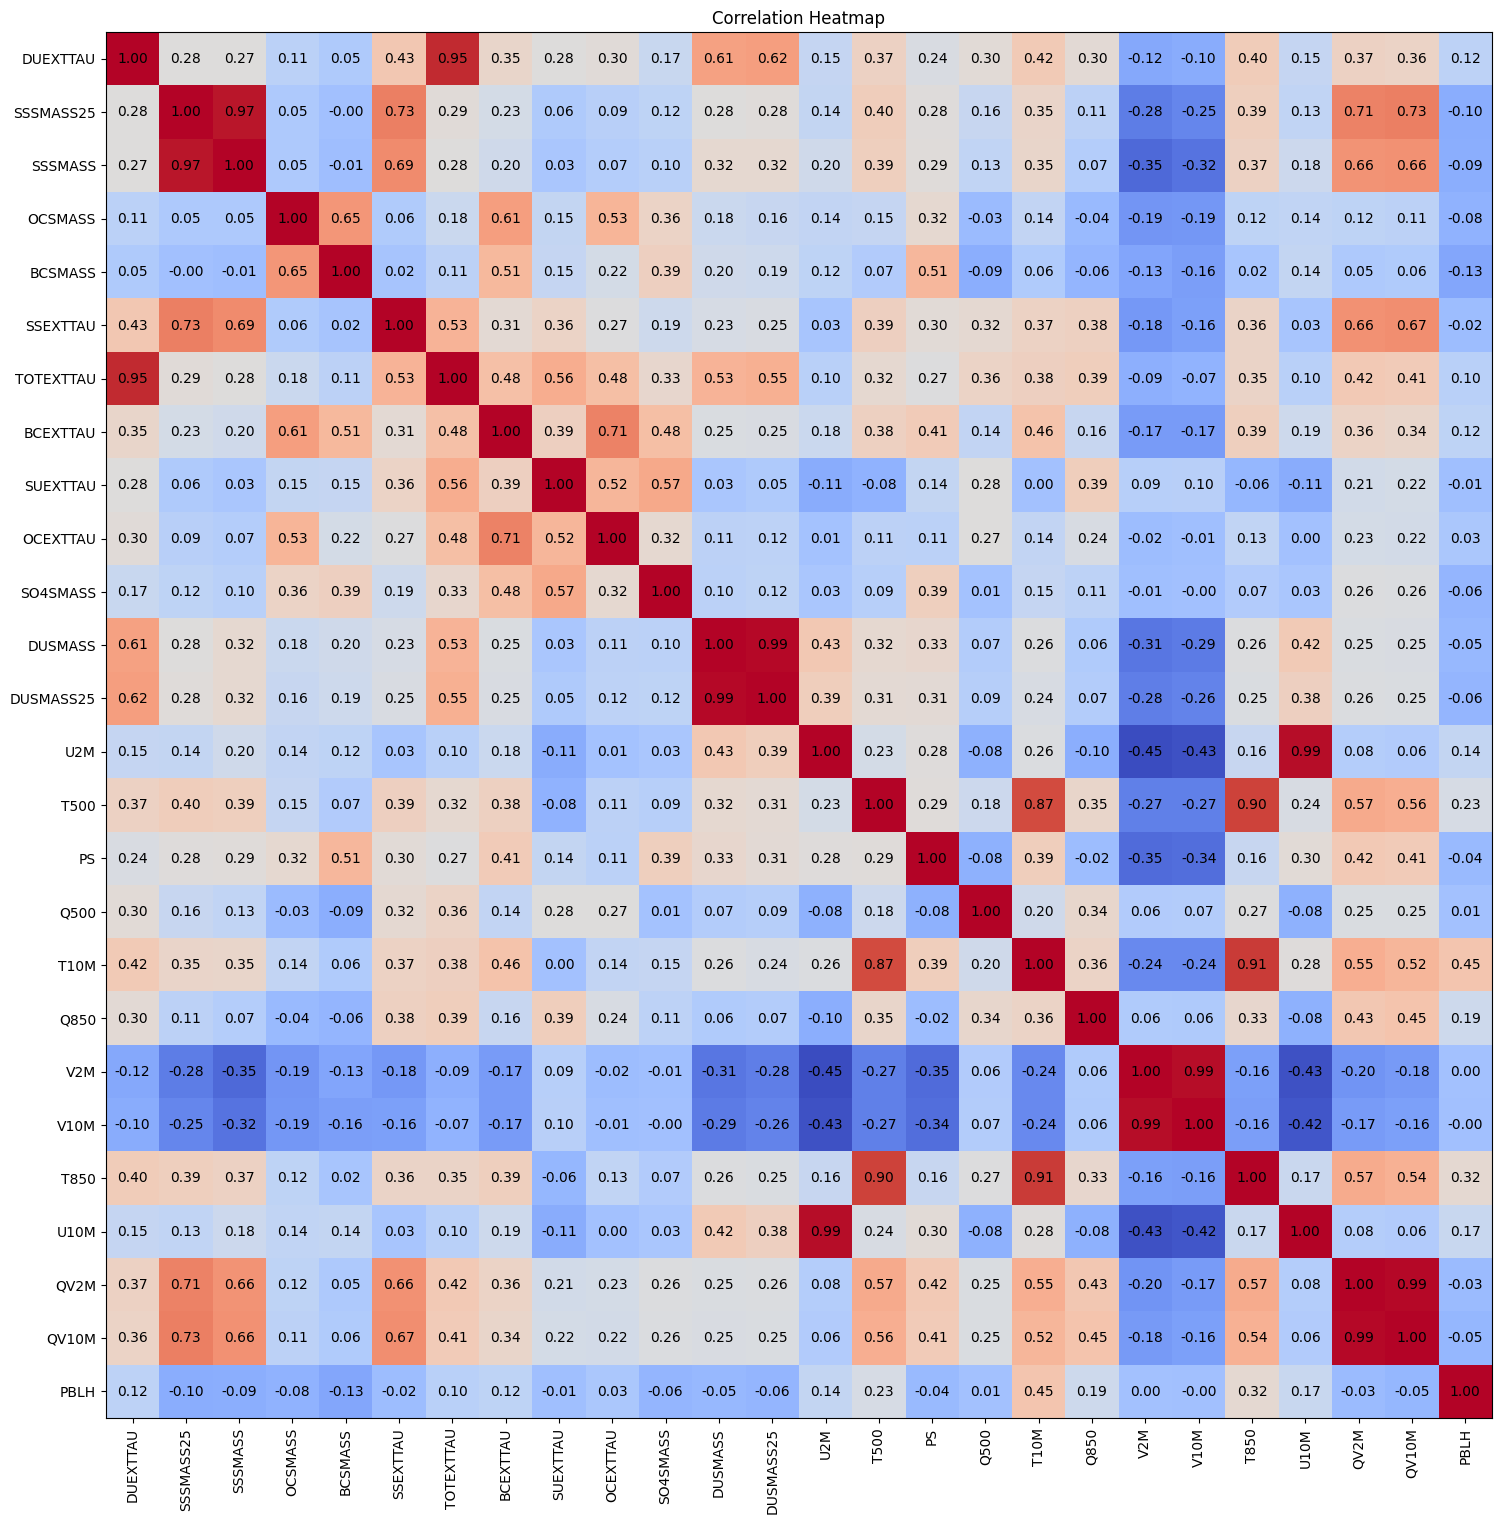
\includegraphics[width=\textwidth]{calibration/correlations.png}
    \caption{MERRA-2 Variable Correlations}
    \label{fig:correlations}
\end{figure}

\textit{Figure \ref{fig:correlations}} shows that there are indeed pairs of variables that are highly correlated. In linear regression, these high correlations would pose severe problems of high variance inflation factors and render incorrect models, and might be a problem here as well. Further studies should omit the highly correlated variables and check whether the results might be better.

\subsubsection{Time Series Data}

For the sake of improving model performance of the predictions, we preprocessed the data to incorporate a temporal lag of 24 for the MERRA-2 variables for every time step so that our models not only have the current time but also past information to predict PM2.5. As such, we introduced LSTMs into our models, a recurrent neural network architecture that reads sequential data to make predictions. As the trending architecture, transformers were also built and compared with LSTMs on the PM2.5 prediction task.

During the training process, we discovered that the loss function for the models largely determined model performance. Throughout the study, we compared multiple loss functions and logged the validation RMSE of the LSTM models in \textit{Table \ref{tab:loss_fn}} below.

\begin{table}[htbp]
    \centering
    \begin{tabular}{l c}
        \toprule
        \textbf{Loss Function} & \textbf{Validation RMSE} \\
        \midrule
        \textit{Baseline (One-Step Model)} & \textit{24.393} \\
        MSE Loss & 22.91 \\
        Weighted MSE & 28.62 \\
        Huber Loss & 22.72 \\
        Pinball Loss & \textbf{21.40} \\
        \bottomrule
    \end{tabular}
    \caption{Validation RMSE on Different Loss Functions}
    \label{tab:loss_fn}
\end{table}

Note that pinball loss has the lowest validation among the four loss functions used. To use the pinball loss function, the LSTM models have been modified to include four heads in the output layer, each predicting the 0.5 quantile, the 0.9 quantile, the 0.95 quantile, and the 0.99 quantile, respectively. Upon finishing training the quantile LSTM models, the final predictions were then taken to be the 0.5 quantile. As mentioned previously, a major problem of the one-step prediction models was that the models underestimated many of the values that were expected to be greater than 500 \( \mu g/m^3 \). Adding higher quantiles during training thus helped the models to capture the greater PM2.5 values so that performance improved.

The mathematical equations for the loss functions are shown below:

\begin{align*}
    \text{MSE}(y, p) &= \frac{1}{n} \sum_{i=1}^{n} (y_i - p_i)^2 \\
    \text{WeightedMSE}(y, p) &= \frac{1}{n} \sum_{i=1}^{n} \left( 1 + \left( \frac{y_i}{500} \right)^2 \right) \times (y_i - p_i)^2 \\
    \text{HuberLoss}(y, p, \delta) &= \begin{dcases}
        0.5(y_i - p_i)^2 & \text{if } |y_i - p_i| < \delta \\
        \delta \cdot |y_i - p_i| - 0.5\delta^2 & \text{otherwise}
    \end{dcases} \\
        \text{PinballLoss}_\tau(y, p) &= \begin{dcases}
            \tau(y_i - p_i) & \text{if } y_i \geq p_i \\
            (1 - \tau)(p_i - y_i) & \text{otherwise}
        \end{dcases}
\end{align*}

In addition to LSTM models, we also built transformers and variational autoencoders that were based on transformers and LSTMs. However, these models did not work as good as expected (worse than the LSTM model with pinball loss) and unfortunately the training logs were lost. Hence the results were not present here.

Transfer learning is a powerful technique in training neural networks. In the current study, we referenced the project conducted by Wang et al. (2022), in which the researchers utilized transfer learning for the MERRA-2 downscaling task. In the paper, the researchers developed an LSTM neural network architecture that had two process blocks consisted of solely fully-connected layers, two temporal blocks consisted of LSTM layers, and a transfer block where there was a transfer model trained on predicting MERRA-2 variables. The rationale was that by pre-training a model to understand the MERRA-2 data, the final downscaling model would have better information in the distribution of the MERRA-2 data in order to make better predictions. In the current study, we replicated the same model architecture and pre-trained a transfer model on the MERRA-2 data to predict itself. Nevertheless, as we applied the final model with the transfer block on the PM2.5 prediction task, we did not obtain great results and so the idea was later abandoned.

In summary, in this section of the project, we developed an LSTM model using the pinball loss and achieved a final validation RMSE of 21.40, which was the lowest among all the models. The \( R^2 \) value was also around 0.80, which was slightly higher than the one-step prediction model.

\subsubsection{Out-of-Sample Validation}

Upon obtaining the final LSTM model, we deployed the model on a daily PM2.5 dataset in Kuwait in the period of 2004-2005 to assess the generalizability of the model. Since the overall objective of the current study is to downscale MERRA-2 from 2002 to 2016, the accuracy of the calibration model in this period is necessary for the accuracy of the downscaling.

The bad news is that the model is not very generalizable. On the 2004-2005 Kuwait PM2.5 dataset, the model achieved an RMSE of only {blank} and an \( R^2 \) of {blank}, which show the poor performance.

\subsection{Conclusion}

In conclusion, on the OpenAQ PM2.5 dataset, our developed model was capable of predicting PM2.5 quite accurately using the MERRA-2 data. The final RMSE of 21.40 and \( R^2 \) of around 0.8 proved the capability of the LSTM model. However, the model is not ready to use for the downscaling task that will be carried out later, as the model was not generalizable to the 2004-2005 Kuwait dataset by only having an RMSE of {blank} and an \( R^2 \) of {blank}.

\subsubsection{Limitations}

There were several limitations associated with the study. The most important one must be the problem with the Kuwait dataset that we used to validate our LSTM model. The data that we trained our models on was hourly in both the PM2.5 and MERRA-2, while the Kuwait validation data was daily. To make up for this incompatibility, we had to average the MERRA-2 data used in the validation to a daily level so that we could hopefully predict the daily PM2.5 values accurately. However, this method is obviously not justified, but we unfortunately did not have applicable hourly PM2.5 data to validate our model on. Future researchers preferably should have more PM2.5 data in the period of 2002 to 2016 to validate the calibration model so that the downscaling portion can be more accurate.

\pagebreak

\section{Appendices}

\subsection{Data}
    \subsubsection{List of MERRA-2 Aerosols Variables}
    \begin{itemize}
        \item \textbf{BCEXTTAU} -- black carbon
        \item \textbf{DUEXTTAU} -- dust
        \item \textbf{SUEXTTAU} -- SO\(_4\)
        \item \textbf{OCEXTTAU} -- organic carbon
        \item \textbf{SSEXTTAU} -- sea salt
        \item \textbf{TOTEXTTAU} -- total aerosol
        \item \textbf{DUSMASS25} -- dust PM2.5
        \item \textbf{SSSMASS25} -- sea salt PM2.5
        \item \textbf{DUSMASS} -- dust
        \item \textbf{BCSMASS} -- black carbon
        \item \textbf{SO4SMASS} -- SO\(_4\)
        \item \textbf{SSSMASS} -- sea salt
        \item \textbf{OCSMASS} -- organic carbon
    \end{itemize}
        
    \subsubsection{List of MERRA-2 Meteorology Variables}
    \begin{itemize}
        \item \textbf{PS} -- surface pressure
        \item \textbf{Q500} -- specific humidity at 500 hPa
        \item \textbf{Q850} -- specific humidity at 850 hPa
        \item \textbf{T850} -- air temperature at 850 hPa
        \item \textbf{T500} -- air temperature at 500 hPa
        \item \textbf{T10M} -- 10-meter air temperature
        \item \textbf{QV10M} -- 10-meter specific humidity
        \item \textbf{QV2M} -- 2-meter specific humidity
        \item \textbf{U10M} -- 10-meter eastward wind
        \item \textbf{U2M} -- 2-meter eastward wind
        \item \textbf{V10M} -- 10-meter northward wind
        \item \textbf{V2M} -- 2-meter northward wind
        \item \textbf{PBLH} -- planetary boundary layer height
    \end{itemize}

    \subsubsection{Location}
    \begin{itemize}
        \item Baghdad, Iran (2 sites)
        \item Manama, Bahrain
        \item Doha, Qatar
        \item Dubai, UAE
        \item Kuwait City, Kuwait
        \item Osh, Kyrgyzstan
        \item Dushanbe, Tajikistan (2 sites)
        \item Ashgabat, Turkmenistan
        \item Tashkent, Uzbekistan
    \end{itemize}

\subsection{Methodology}

\begin{enumerate}
    \item Pulled ground-level measurements from OpenAQ
    \item Pulled MERRA-2 data
    \item Matched OpenAQ and MERRA-2 data by location and time
    \item Replicated Sayeed et al. (2022) paper by evaluating OLS, Ridge, Lasso, Stochastic Gradient Descent, KNN, SVM, Ada Boost, Gradient Boosting, Decision Tree, Random Forest, NN, and XGBoost on a 10\% subset of data
    \item Tried different neural networks, training hyperparameters, and feature engineering
    \item \textbf{Feature Engineering Steps:}
    \begin{enumerate}
        \item Only MERRA-2 variables for prediction
        \item Added cyclical encoding for month, day, and hour
        \[\text{value}_{\sin}(x) = \sin \left(\frac{2\pi x}{\text{max value}}\right) \]
        \[\text{value}_{\cos}(x) = \cos \left(\frac{2\pi x}{\text{max value}}\right)\]
        For example, the max value for month is 12.
        \item Added one-hot vector for sites
        \item Changed site information into embeddings using an embedding layer in PyTorch, \(\dim = 256\)
        \item Added season information, also as embeddings, \(\dim = 32\)
        \item Used embeddings for all of site, season, hour, day, month, removed cyclical embeddings
        \item Added aridity information, also as embeddings \(\dim = 200\)
    \end{enumerate}
\end{enumerate}

\pagebreak

\end{document}
